% !TEX TS-program = XeLaTeX
\documentclass{CSICC2020}

% تقریبا تمامی بسته‌های مورد نیاز برای یک مقاله در استایل فراخوانی شده است. اما در هر صورت در صورتی‌که می‌خواهید بسته‌ای را فراخوانی کنید به صورت زیر عمل کنید. مثلا ما در کد زیر دوبسته glossaries و tikz را فراخوانی کرده‌ایم.
%\makeatletter
%\bidi@BeforePackage{xepersian}{
	%\RequirePackage{tikz}
	%\RequirePackage{glossaries}
	%}
%\makeatother


% عنوان مقاله را در این قسمت وارد کنید. 
\title{
	طبقه بندی URL های مخرب با استفاده از Bayes Naive و الگوریتم ژنتیک
}
\date{}
% اسامی نویسندگان و همچنین اطلاعات مربوط به آن‌ها را در این قسمت وارد کنید. 
\author[1]{مورات کوجا}
\author[2]{عیسی آوجی}
\author[2]{محمد عبدالکریم شکیر الحیانی }
\affil[1]{
	 دانشگاه ییل یوزونجو وان، دانشکده مهندسی کامپیوتر
}
\affil[2]{
	دانشگاه کارابوک، دانشکده مهندسی کامپیوتر 
}

%\cite{islam2019using}
\begin{document}
	\maketitle
	\begin{abstract}
		زیان‌های مالی وب‌سایت‌های آسیب‌پذیر و ناامن روز به روز در حال افزایش است. سیستم پیشنهادی در این مقاله، یک استراتژی‌ مبتنی بر تحلیل عاملی دسته‌بندی‌های وب‌سایت‌ و شناسایی دقیق اطلاعات ناشناخته را ارائه می‌دهد تا وب‌سایت‌های ایمن و خطرناک را طبقه‌بندی کرده و کاربران را از وب‌سایت‌های ناامن محافظت کند. در طول فرآیند طبقه‌بندی وب‌سایت، از محاسبات احتمالی مبتنی بر \lr{Naive Bayes} و سایر روش‌های قدرتمند استفاده می‌شود تا مدل طبقه‌بندی وب‌سایت ارزیابی و آموزش داده شود. طبق مطالعه ما، روش \lr{Naive Bayes} نتایج موفقیت‌آمیزی را نسبت به سایر آزمایش‌ها نشان می‌دهد. این استراتژی بهترین بهینه‌سازی را برای حل مشکل تمایز وب‌سایت‌های ایمن از ناامن ارائه می‌دهد. مدل آموزش دسته‌بندی داده‌های آسیب‌پذیری در این دیتاشیت، دقت بالاتری را نشان داد. در این مطالعه، بهترین دقت احتمالی ۹۶٪ در دسته‌بندی داده‌های مجموعه  \lr{Naive Bayes' NSL-KDD} به دست آمد.
	\end{abstract}
	\begin{keywords}
		شبکه عصبی، یادگیری ماشین، \lr{Naive Bayes}، مخرب، \lr{HTML}  
	\end{keywords}
	
	\section{مقدمه}
	\label{sec:introduction}
	
	هکرها از وب‌سایت‌های تجاری و تبلیغات تصادفی برای انتشار لینک‌های مخرب خود استفاده می‌کنند \cite{tavallaee2009detailed}. زیرا کاربران اینترنت باور دارند که مشارکت آن‌ها منجر به سود مالی خواهد شد. آنها قربانی طرح‌های کلاهبرداری می‌شوند، همانند آن‌هایی که وام‌های جعلی تبلیغ می‌کنند، یا کالاهای ارزان‌قیمت می‌فروشند. برای جلوگیری از آسیب‌های فیزیکی و  وب‌سایت‌هایی که خطراتی علیه امنیت ما دارند، تخصص کافی لازم نیست \cite{sharma2020malicious}.\\
	
	تبلیغات به دلایل مختلف وجود دارد، اما هدف نهایی آن‌ها این است که افراد را ترغیب کند تا روی لینک‌ها و تبلیغات مرتبط کلیک کنند تا بتوانند محتوا را بخوانند. در سال ۲۰۱۹، Symantec گزارشی درباره امنیت اینترنت منتشر کرد که در آن این شرکت به وجود حملات گسترده و متوالی به شرکت‌ها برای سرقت اطلاعات و ایجاد خسارات قابل توجه، و همچنین تهدیدات بزرگ برای حساب‌های شخصی و بانکی و تهدید قربانیان از طریق پیام‌های تهدیدآمیز برای پرداخت یک باج مشخص با استفاده از روش‌های مختلف اشاره کرد. Symantec همچنین به وجود تهدیدات گسترده برای حساب‌های شخصی و مالی، و همچنین خطر دریافت درخواست‌های باج از قربانیان اشاره کرد. با کلیک کردن روی لینک‌های مخرب در تبلیغات گمراه‌کننده (کلاهبرداری)، افراد به وب‌سایت‌های خصمانه هدایت می‌شوند \cite{santoshi2021twitter}.\\
	
	در حال حاضر، تکنیکی که برای حمله به یک شبکه استفاده می‌شود، نیز توسعه‌ یافته و دشواری حفاظت از شبکه‌های جهانی با همان سرعت رشد اقتصاد در حال تشدید است. طبق پیش‌بینی‌ها، انتظار می‌رود که بازار امنیت شبکه، نشانه‌هایی از رشد را در حدود سال ۲۰۲۱ نشان دهد \cite{islam2019using}.\\
	%picture
	\begin{figure}
		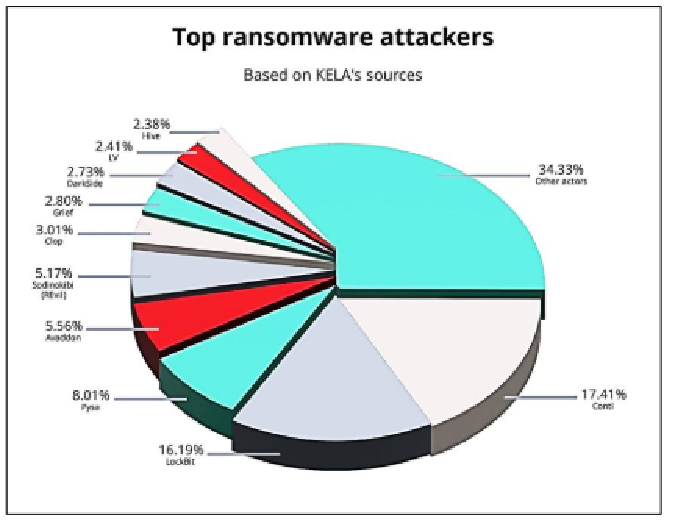
\includegraphics[width=.9\linewidth]{Images/related.pdf}
		\caption{
			نسبت حملات در لینک‌های مخرب \cite{santoshi2021twitter}}
		\label{fig:sumXYPlot}
	\end{figure}
	تحقیقات نشان می‌دهد که حفاظت و حفظ یکپارچگی چنین شبکه‌هایی با توجه به افزایش فراوانی حملات مجرمان سایبری به شبکه‌ها به یک هدف بسیار مهم تبدیل شده است. این به این دلیل است که مجرمان سایبری به طور فزاینده‌ای شبکه‌ها را هدف قرار می‌دهند که منجر به وضعیت کنونی شده است که سیستم پیشنهادی خود را در آن می‌یابد. اکثر مردم در طول یک روز عادی، به تعداد زیادی از \lr{URL}های اینترنتی مراجعه می‌کنند. این فعالیت معمولاً به عنوان بخشی از فعالیت‌هایی که یک روز عادی را تشکیل می‌دهند، محسوب می‌شود. متاسفانه، در این تعداد زیاد و رو به افزایش \lr{URL}ها، اکنون تعداد قابل توجهی از \lr{URL}ها وجود دارند که به وب‌سایت‌های خطرناک متصل می‌شوند که یک روند بسیار نگران‌کننده است. به دلیل رشد سریع اینترنت، ورود اشتباهی به \lr{URL}های مضر به جای \lr{URL}های قانونی بسیار آسان شده است. به دلیل اینکه امکان اشتباه گرفتن \lr{URL}های مخرب با \lr{URL}های معتبر وجود دارد، انجام این اشتباه دشوار نیست. در نتیجه ، بسیار ضروری است که توانایی‌های لازم برای تمایز سریع و دقیق بین این دو را پرورش دهیم \cite{oyelakin2023performance}. \\
	هدف جامعه علمی، شناسایی \lr{URL}هایی است که پتانسیل رفتارهای کلاهبرداری دارند و برای این منظور، از مدل‌های معیار مختلفی استفاده می‌کنند. سیستم پیشنهادی از یک مجموعه داده که شامل رخدادهای \lr{URL} بود استفاده کرد تا عملکرد \lr{SVM (Support Vector Machine)} ،lr{KNN (K-Nearest Neighbors)} و درخت \lr{Naive Bayes} را ارزیابی کند. به عنوان نتیجه این مطالعات، سیستم پیشنهادی دریافت که استفاده از این فناوری دقت \lr{SVM} و \lr{KNN} را در طبقه‌بندی داده‌ها افزایش داده است.  دریافتیم که \lr(Decision Tree) در مقایسه با سایر روش‌ها کمترین درجه اثربخشی را داشته است. گفته شده است که یک طبقه‌بند بیز ساده می‌تواند به عنوان ابزاری برای طبقه‌بندی و تعیین خودکار \lr{URL}هایی که پتانسیل جعلی بودن دارند، استفاده شود. این می‌تواند از طریق استفاده از یک برنامه کامپیوتری انجام شود. در مجموعه‌های داده معیار مختلف، عملکرد مدل بیز ساده که با استفاده از یادگیری مدل احتمالاتی آموزش دیده بود، بهتر از مدل \lr{SVM} است \cite{serda2013synteza}.\\
	این در حالی است که مدل \lr{SVM} نیز با استفاده از یادگیری مدل احتمالاتی آموزش دیده بود. این نتیجه از آموزش برای بهبود عملکرد مدل بیز ساده به دست آمده است حتی اگر مدل \lr{SVM} با استفاده از یادگیری مدل احتمالاتی ساخته شده باشد. یک سیستم فیلترینگ چند مرحله‌ای توسعه داده شده که \lr{URL}های بالقوه خطرناک را با استفاده از تکنیک‌های مرتبط با یادگیری ماشین شناسایی می‌کند، که یک زمینه تحقیقاتی به اختصار \lr{ML} است \cite{serda2013synteza}.\\
	این بر اساس تکنیک‌های مرتبط با یادگیری عمیق است که به اختصار یادگیری عمیق نامیده می‌شود. از آنجا که طبقه‌بند با آستانه بحرانی آموزش دیده است، اکنون امکان دارد طبقه‌بند بر \lr{URL}هایی که عملکرد بسیار خوبی دارد تمرکز کند و آن‌ها را شناسایی کند. این یک اثر مستقیم از آموزش طبقه‌بند با آستانه بحرانی است. به همین دلیل، طبقه‌بند می‌تواند با بالاترین سطح کارایی خود عمل کند. اگر متوجه شدید که گروه خاصی از طبقه‌بندها قادر به تخصیص صحیح یک \lr{URL} به یکی از دسته‌های خود نیستند، باید با تعدادی از طبقه‌بندها رأی دهید. در نهایت، مهم است که تأکید شود که دقت شناسایی \lr{URL}های مخرب با استفاده از این روش در مقایسه با مدل بیزی، مدل \lr{Decision Tree}، و مدل SVM افزایش یافته است. برای طبقه‌بندی صحیح \lr{URL}های بالقوه خطرناک، رگرسیون لجستیک، شبکه‌های عصبی، و سه تکرار مختلف از روش بیز ساده به عنوان ابزار تحلیلی استفاده شد. طبق نتایج مطالعه، استراتژی‌های بیز ساده آن‌هایی بودند که بالاترین نرخ موفقیت را داشتند. شیخ شاه محمد مطیعور اثربخشی تعداد زیادی از طبقه‌بندهای یادگیری ماشین را ارزیابی کرد تا تعیین کند آیا آن‌ها قادر به شناسایی صحیح \lr{URL}های فیشینگ هستند یا خیر \cite{wu2022classification}.\\
	معیارهایی که او برای ارزیابی اثربخشی این طبقه‌بندها استفاده کرد شامل مساحت زیر منحنی مشخصه عملکرد گیرنده (AUC-ROC)، دقت، نرخ نادرست طبقه‌بندی، و میانگین خطای مطلق بودند. در مورد طبقه‌بندی دودویی و مجموعه ویژگی‌هایی که چندین کلاس مختلف را شامل می‌شوند، تعمیم پشته‌ای نتایج دقیق‌تری را نسبت به جنگل تصادفی و پرسپترون چندلایه ارائه می‌دهد. تأثیر بسزایی که استفاده از تعداد زیادی مدل‌های یادگیری ماشین، به‌ویژه مجموعه‌های \lr{ML}، برای حل مشکل یافتن \lr{URL}های جعلی دارد. جنگل تصادفی نتیجه یادگیری ارثی است و چندین معیار، از جمله نرخ یادآوری، نرخ دقت، و مقدار مساحت زیر منحنی (\lr{AUC})، نشان داده‌اند که برتری نسبت به مدل \lr{ML} متداول دارد. شبکه‌های عصبی پیچشی (\lr{CNN})، شبکه‌های حافظه طولانی‌مدت کوتاه (\lr{LTSM})، و شبکه‌های عصبی پیچشی-حافظه‌ای (\lr{CNN-\lr{LTSM}}) سه نوع مختلف از شبکه‌های عصبی عمیق بودند که در فرآیند شناسایی \lr{URL}های جعلی استفاده شدند \cite{rajalakshmi2019transfer}.\\
	
	با این حال، برای پیشنهاد یک مدل شبکه عصبی پیچشی بازگشتی چندلایه الهام‌گرفته از \lr{YOLO} برای شناسایی \lr{URL}های مخرب، آن‌ها مقایسه‌ای از لایه پنهان و تعداد نورون‌ها در آزمایش انجام ندادند. اختصارات (\lr{CNN})، (\lr{LTSM})، و (\lr{CNN-LTSM}) سه اختصاری هستند که بیشتر استفاده می‌شوند. مدل‌های \lr{Text-RCNN} و \lr{BRNN}، به همراه بسیاری از روش‌های دیگر، نمی‌توانند با سطح دقتی که با استفاده از این روش می‌توان به دست آورد، رقابت کنند. در طول مطالعه، هر \lr{URL} به طور دقیق به همان روش کوتاه خواهد شد تا همگی به یک طول برسند. این فرآیند تکرار خواهد شد تا هیچ تمایزی بین آن‌ها باقی نماند \cite{wejinya2021machine}. کار با \lr{URL}های طولانی‌تر شما را در معرض خطر بیشتری از دست دادن داده‌ها نسبت به انجام همین فعالیت با \lr{URL}های کوتاه‌تر قرار می‌دهد. یک رابطه یک به یک بین طول \lr{URL} و شدت این خطر وجود دارد. استفاده از مدل یادگیری ماشین معیار به عنوان یک گام در فرآیند توسعه استراتژی‌های مهندسی ویژگی پیشرفته‌تر برای افزایش نرخ شناسایی \lr{URL}های بالقوه مضر یک امکان است.\\
	
	این کار به منظور افزایش نرخ شناسایی \lr{URL}های بالقوه مضر انجام می‌شود. روشی برای مهندسی ویژگی ایجاد شد که می‌تواند مختصات فضایی شیء تولید شده را به صورت خطی یا غیرخطی تغییر دهد، بسته به نوع تغییری که سیستم پیشنهادی می‌خواهد انجام دهد. هر دوی این کاربردها گزینه‌های قابل قبولی برای استفاده از این فناوری هستند. نرخ‌های شناسایی \lr{KNN}، \lr{SVM} خطی، و پرسپترون چندلایه به طور قابل توجهی بهبود می‌یابد هنگامی که پنج مدل تبدیل فضایی مجزا برای تولید و اعمال ویژگی‌های اضافی به طبقه‌بند استفاده شوند. این به این دلیل است که طبقه‌بند اکنون شامل تعداد بیشتری ویژگی است. تولید قابلیت‌ها و ویژگی‌های جدید با کمک این پنج مدل انجام می‌شود.\\
	استخراج اطلاعات از متنی که درون \lr{URL} گنجانده شده است، تمرکز اصلی اکثر روش‌هایی است که امروزه برای شناسایی \lr{URL}های جعلی می‌توان از آن‌ها استفاده کرد. این امر برای اکثر روش‌های مختلف صادق است. سیستم پیشنهادی یک روش داده‌کاوی مبتنی بر طبقه‌بندی ارتباطی برای شناسایی \lr{URL}های مضر بر اساس \lr{URL}ها و ویژگی‌های استخراج شده از محتوای آنلاین ارائه می‌دهد. این روش روابط بین \lr{URL}ها و ویژگی‌ها را تحلیل می‌کند. این رویکرد از خود \lr{URL}ها به همراه ویژگی‌هایی که ممکن است از \lr{URL}ها استخراج شوند، استفاده می‌کند. این استراتژی ترکیبی از استفاده از طبقه‌بندی و قوانین ارتباطی را به کار می‌گیرد تا به آنچه لازم است دست یابد. مجموعه‌ای از دستورالعمل‌ها که وقتی ترکیب می‌شوند، امکان قرار دادن چیزها در دسته‌ها و ایجاد روابط بین آن‌ها را فراهم می‌کنند \cite{alzubaidi_detect}.
	
	سیستم پیشنهادی ابتدا یک رویکرد وزنی ارائه می‌دهد که مجموعه‌ای اساسی از ویژگی‌ها را برای مطالعه استخراج می‌کند، و سپس سیستم پیشنهادی الگوریتم‌های یادگیری ماشین را بر اساس سرعت و کارآیی آن‌ها در یادگیری ارزیابی می‌کند. این کار برای افزایش درک ما از موضوع انجام می‌شود. این روش اطلاعات واژگانی را از \lr{URL}ها جمع‌آوری کرده و سپس به سادگی آن‌ها را تحلیل می‌کند تا لینک‌های مخرب را پیدا کند. الگوریتم جنگل تصادفی و الگوریتم \lr{KNN} هر دو پتانسیل تولید نتایج مثبت از تحقیقات را دارند. کشف شد که روش خالص واژگانی توانایی امکان تعیین سریع و بلادرنگ \lr{URL}ها در سیستم‌های سبک را دارد \cite{el-din2021malweb}.
	
	این امر با جمع‌آوری ویژگی‌های واژگانی استاتیک از رشته‌های \lr{URL} و سپس طبقه‌بندی آن‌ها با استفاده از یک الگوریتم طبقه‌بندی مجموعه‌ای که توسط یادگیری ماشین آموزش دیده است، انجام می‌شود.این روش بارها و بارها تکرار می‌شود تا نتیجه مطلوب حاصل شود. روشی برای شناسایی توسعه داده شد که کاملاً به ویژگی‌های واژگانی محتوایی که به دنبال کشف آن هستند، وابسته است. شبکه عصبی پیچشی اکنون در موقعیتی است که می‌تواند نتیجه طبقه‌بندی دقیق‌تری ارائه دهد زیرا رشته‌های \lr{URL} جمع‌آوری و پردازش شده‌اند. به عنوان نتیجه مستقیم افزایش دقت طبقه‌بندی، این امر اکنون امکان‌پذیر است. مدل تکنیک شبکه عصبی ترکیبی را با ترکیب \lr{BI-Ind RNN} و \lr{Caps Net} برای شناسایی \lr{URL}های مخرب، استخراج ویژگی‌ها (شامل ویژگی‌های برداری و بافتی در سطح کاراکتر و کلمه) و ترکیب ویژگی‌ها توسعه داد \cite{wang2020auto1}.
	
	این مدل به طور خاص برای شناسایی \lr{URL}های مخرب ایجاد شده است. وقتی یک شبکه عصبی ترکیبی برای فرآیند طبقه‌بندی استفاده می‌شود، نه تنها سرعت شناسایی \lr{URL}های بالقوه مضر به طور قابل توجهی افزایش می‌یابد بلکه دقت شناسایی آن‌ها نیز به طور قابل توجهی افزایش می‌یابد. \lr{URL‌ Net} یک شبکه عصبی عمیق مبتنی بر CNN است که برای تعیین اینکه آیا یک \lr{URL} جعلی است یا خیر، توسعه یافته است. نام این شبکه از عبارت "\lr{universal resource locator}" گرفته شده است که عملکرد آن را توصیف می‌کند. \lr{CNN} و کلمه "\lr{CNN}" ترویج می‌شوند و شبکه برای مدیریت محدودیت‌های مهندسی ویژگی دستی و عدم شفافیت در \lr{URL}های آزمون تنظیم شده است \cite{wang2020auto2}.
	\section{کارهای مرتبط}
	تحقیقات زیادی درباره دشواری دسته‌بندی تعداد زیادی از وب‌سایت‌های موجود انجام شده است. طبقه‌بند \lr{Naive Bayes}، که معمولاً برای توسعه راه‌حل‌های با کیفیت بالا برای مشکلات جستجو با استفاده از اپراتورهای الهام‌گرفته از زیست‌شناسی استفاده می‌شود، می‌تواند با الگوریتم ژنتیک ترکیب شود که معمولاً برای کاهش زمان پردازش با توسعه راه‌حل‌های با کیفیت بالا برای مشکلات جستجو با استفاده از اپراتورهای الهام‌گرفته از زیست‌شناسی استفاده می‌شود \cite{fadheel2022phishing}. طبقه‌بند \lr{Naive Bayes} قادر خواهد بود راه‌حل‌های با کیفیت بالا برای مشکلات جستجو با استفاده از اپراتورهای الهام‌گرفته از زیست‌شناسی توسعه دهد. استفاده از اپراتورهای الهام‌گرفته از زیست‌شناسی به این روش به طبقه‌بند \lr{Naive Bayes} اجازه می‌دهد تا راه‌حل‌های با کیفیت بالا برای مشکلات جستجو تولید کند. علاوه بر این، این ترکیب می‌تواند کل زمان مورد نیاز برای فرآیند را کاهش دهد. آن‌ها انواع مختلفی از عملکردهای اضافی علاوه بر قابلیت‌های مبتنی بر واژگان و میزبان ارائه می‌دهند. این ویژگی‌ها شامل قابلیت فعال یا غیرفعال کردن \lr{JS}، محتوای یک عنصر \lr{HTML}، و بسیاری دیگر است. زمان پردازش اضافی برای دسته‌بندی صفحات وب مورد نیاز است زیرا ۳۱ ویژگی مختلف قابل استفاده برای انجام این کار وجود دارد \cite{liu2017analysis}.
	
	از سوی دیگر، امکان سازماندهی صفحات وب وجود دارد. در نتیجه این، امکان دسته‌بندی وب‌سایت‌ها بر اساس طیف گسترده‌ای از ویژگی‌های مختلف وجود دارد. آن‌ها از طیف وسیعی از تاکتیک‌ها، مانند سوئیچینگ ویژگی تکراری و بهینه‌سازی مبتنی بر \lr{Genetic Algorithm (GA)}، برای دستیابی به سطح دقت مطلوب استفاده کردند و در انجام این کار موفق بودند \cite{subasi2021comparative}. محققان مشاهده کردند که با استفاده از طبقه‌بند \lr{Naive Bayes} برای شناسایی وب‌سایت‌ها بر اساس ویژگی‌های \lr{URL}، توانستند نرخ دقت ۷۸٪ را با استفاده از این استراتژی به دست آورند. این یک افزایش قابل توجه در دقت در مقایسه با نرخ‌های قبلی آن‌ها بود که بدون \lr{GA} ۷۴٪ و با \lr{GA} ۸۷٪ بود. این نشان‌دهنده افزایش ۳٪ نسبت به سال قبل بود. آن‌ها تلاش خود را بر روی کشف نحوه استفاده مردم از وب‌سایت‌ها متمرکز کرده‌اند و مجموعه داده‌ای که از آن استفاده می‌کنند بسیار جامع است. یک منبع اصلی ناامیدی این است که دقت کلی کمتر از چیزی است که انتظار می‌رفت، حتی اگر میانگین تعداد یادآوری‌ها بالاتر از ۸۸٪ باشد. این به این دلیل است که میانگین تعداد یادآوری‌ها بالاتر از ۸۸٪ است.
	
	این رفتار شامل تظاهر به یک وب‌سایت دیگر برای سرقت اطلاعات حساس از کاربران آن است. حتی اگر پروژه‌هایی که روی آن‌ها کار می‌کنند به طور خاص برای یافتن وب‌سایت‌های جعلی طراحی نشده باشند، استراتژی‌هایی که برای انجام این کار استفاده می‌کنند، به خودی خود مهم هستند. آن‌ها توانستند دقت نهایی ۸۹.۱٪ و ۸۸.۵٪ را با روش جنگل چرخشی به دست آورند که ثابت می‌کند این بهترین الگوریتم پس از انجام آموزش و آزمایش‌های گسترده است. پس از نصب رتبه‌بندی ویژگی، آن‌ها موفق شدند دقت ۸۹٪ با استفاده از \lr{MLP} و دقت ۸۷/۵٪ با استفاده از \lr{REP Tree} به دست آورند. هر دو این نتایج پس از معرفی رتبه‌بندی ویژگی حاصل شدند. کشف شده است که استفاده از پرسپترون‌های چندلایه، که یکی از دسته‌های شبکه‌های عصبی مصنوعی پیش‌خور هستند، نتایج موفقیت‌آمیزی را که در تحقیقات قبلی به دست آمده است، به همراه دارد. به دلیل این شبکه، تعداد ابعادی که داده‌ها از آن تشکیل شده‌اند به طور قابل توجهی کاهش می‌یابد. اگر محققان از جنگل چرخشی در کل مجموعه آموزشی استفاده کنند، احتمال زیادی وجود دارد که بهبود قابل توجهی در حاشیه دقت خود به دست آورند. این به این دلیل است که جنگل چرخشی یک روش برای یادگیری تحت نظارت است، که توضیح می‌دهد چرا این نتایج به دست آمدند. جنگل چرخشی الگوریتم‌های دیگر، مانند جنگل تصادفی و درخت تصادفی فوق‌العاده \cite{sharma2020malicious}، را در برنامه‌های عملیاتی شکست می‌دهد زیرا با استفاده از تعداد کمتری درخت، تعداد بیشتری از نتایج را تولید می‌کند. این دلیل اصلی برتری جنگل چرخشی است.
	
	
	به عبارت دیگر، کارآیی روش جنگل چرخشی بسیار بالاتر است. با این حال، پیچیدگی الگوریتم‌های آن‌ها و مدت زمان لازم برای اجرای دستورات آن‌ها همچنان موانعی خواهند بود. \lr{SVM}، J48، \lr{Naive Bayes}، و رگرسیون لجستیک از جمله روش‌هایی هستند که باید هنگام جستجوی وب‌سایت‌ها برای بدافزار مورد استفاده قرار گیرند. این‌ها فقط چند گزینه موجود هستند. آن‌ها تعدادی از طبقه‌بندهای تک لایه مختلف را ارزیابی کردند و به این نتیجه رسیدند که \lr{MLP} موثرترین روش برای شناسایی وب‌سایت‌هایی است که ممکن است حاوی محتوای مخرب باشند. به عنوان نتیجه تحقیقات بیشتر، آن‌ها به این نتیجه رسیدند که استراتژی تشخیص لایه متقاطع \lr{XOR-aggregation} برتر از سایرین است زیرا به ندرت نیاز به استفاده از روش‌شناسی پویا دارد \cite{wang2020auto2}. این درک آن‌ها را به این نتیجه رساند که استراتژی تشخیص لایه متقاطع \lr{XOR-aggreagation} برتر از سایرین است.
	
	هنگام استفاده از طبقه‌بند \lr{Naive Bayes}، باید به خاطر داشت که استفاده از ویژگی‌های متعدد منجر به نتایج شناسایی رضایت‌بخش نمی‌شود. اگرچه ممکن بود از یک طبقه‌بند \lr{J48} با لایه متقاطع تجمیع داده برای دستیابی به دقت شگفت‌انگیز 99.178٪ استفاده شود، این فرآیند بیش از چهار دقیقه طول کشید، که ممکن است برای برخی از مشتریان ناراحت‌کننده باشد. به دلیل افزایش فزاینده شبکه‌های اجتماعی و حجم زیادی از داده‌هایی که تولید می‌کنند، کنجکاوی محققان برانگیخته شده است. این به این دلیل است که محققان قادر به مشاهده داده‌های بیشتری نسبت به قبل بوده‌اند. در سال‌های اخیر، مقدار قابل توجهی از تمرکز و تحقیق بر موضوعات مختلف، از جمله شناسایی و فیلتر کردن اسپم، محلی‌سازی جوامع، و انتشار دانش، به عنوان چند نمونه از تجلیات خاص این موضوعات قرار گرفته است.
	
	تعدادی از روش‌های طبقه‌بندی مختلف، مانند\lr{SMO}، \lr{Naive Bayes}، \lr{J48}، و جنگل تصادفی، در فرآیند دسته‌بندی ایمیل‌های اسپم به دسته‌های صحیح استفاده می‌شوند. این‌ها تنها چند استراتژی طبقه‌بندی مختلفی هستند که به کار گرفته می‌شوند. طبق نتایج تحقیق، جنگل تصادفی در مقایسه با روش‌های طبقه‌بندی جایگزین در معیارهای دقت وزنی (۹۵/۵٪)، یادآوری (۹۵/۵٪)، دقت (۹۵/۵٪)، و معیار (۹۵/۵٪) بسیار بهتر عمل می‌کند. پیشنهاد شد که روش تشخیص اسپم \lr{S3D} که در جمله قبلی ذکر شد، می‌تواند به جای روش تشخیص اسپم نیمه‌نظارتی مورد استفاده قرار گیرد. \lr{S3D} از چهار طبقه‌بند سبک وزن منحصر به فرد برای دستیابی به هدف شناسایی توییت‌های اسپم در زمان واقعی استفاده می‌کند. این امر با طراحی مدولار پلتفرم امکان‌پذیر است. نویسندگان مقاله استراتژی‌ای برای شناسایی اسپم‌های توییتر ارائه دادند که به وضعیت روحی فعلی کاربر به عنوان عامل تعیین‌کننده وابسته است \cite{islam2019using}.
	
	این استراتژی برای تعیین احساساتی که در متن بنگالی ذکر شده بود استفاده شد. بر اساس نتایج آزمایش‌هایی که انجام شد، مشخص شده است که روش پیشنهادی قادر است دقت ۷۷/۱۶ درصد را در تشخیص دو احساس اساسی (اندوه و شادی) در متن بنگالی(\lr{‌Bengali text}) به دست آورد. در این آزمایش‌ها، شرکت‌کنندگان موظف به یافتن نمونه‌هایی از احساسات مذکور در یک متن بنگالی بودند. بر اساس نتایج تحقیقی که توسط\lr{Houshmand Craniometry} با استفاده از تعدادی از استراتژی‌های مختلف یادگیری ماشین بر روی مجموعه داده‌های پیامک اسپم که از مخزن یادگیری ماشین \lr{UCI} در دسترس قرار گرفت \cite{sayamber2014malicious}، اعتبارسنجی متقابل ۱۰ برابری بالاترین سطح دقت را تولید کرد \cite{sayamber2014malicious}. این الگوریتم جدید نظارت‌شده یادگیری ماشین را که بر اساس داده‌های رفتاری ساخته شده است به عنوان ابزاری برای شناسایی حساب‌های اسپم در شبکه‌های اجتماعی معرفی می‌کند. این الگوریتم به عنوان روشی برای حذف حساب‌های ناخواسته مورد استفاده نیز قرار می‌گیرد \cite{rajalakshmi2019transfer}. روش توسعه‌یافته در \cite{jian2016design} یافت می‌شود. شناسایی حساب‌هایی که برای اسپم استفاده می‌شوند، نیاز به استفاده از این روش دارد. آن‌ها داده‌های مورد نیاز خود را از \lr{Weibo} جمع‌آوری کردند و سپس از یک روش مبتنی بر \lr{ELM} برای شناسایی حساب‌های اسپم در میان حساب‌های کاربری که به دست آوردند، استفاده کردند.
	
	محتوای متنی، اطلاعات پروفایل کاربر و تعاملات اجتماعی سه نوع ویژگی هستند که باید به ترتیب ارائه شده در اینجا به عنوان بخشی از این تکنیک انتخاب شوند. هر یک از این سه نوع ویژگی از منبعی متفاوت مشتق شده است. این تکنیک برای شناسایی حساب‌های کاربری که برای ارسال اسپم استفاده می‌شدند، اجرا شد. طبق منبع ذکر شده، اثربخشی شناسایی پیامک‌های اسپم پس از افزودن یک ویژگی جدید مبتنی بر محتوا که پیاده‌سازی شده بود، افزایش یافت. یافته‌هایی که از اعمال طیف وسیعی از استراتژی‌های طبقه‌بندی بر روی تعداد زیادی پیام به دست آمد، اعتبار این ادعا را تأیید می‌کند که بهبودهای پیشنهادی منجر به افزایش سطح دقت شناسایی پیامک‌های اسپم خواهد شد. این یافته‌ها پس از اعمال استراتژی‌های طبقه‌بندی مختلف بر روی تعداد زیادی پیام جمع‌آوری شد. علاوه بر این، \cite{alzubaidi_detect} سیستم شناسایی اسپم برای رسانه‌های اجتماعی که مبتنی بر وب و قابل مقیاس است را مورد بحث قرار می‌دهد.
	
	هدف سیستم حفظ اعتماد به شبکه‌های اجتماعی با جلوگیری از ایجاد پست‌ها و نظرات جعلی است. به همین دلیل، آن‌ها توانستند حجم زیادی از داده‌ها را به شیوه‌ای کارآمدتر خوشه‌بندی کنند. نام این الگوریتم‌ها که به عنوان درخت تصمیم، \lr{KNN}، \lr{Naive Bayes} و \lr{SVM} شناخته می‌شوند، معمولاً به عنوان (\lr{SVM}) شناخته می‌شوند. یک شبیه‌سازی آزمایش آموزشی به عنوان وسیله‌ای برای تقلید از بهبود پیشرونده‌ای که ممکن است در فیلترهای اسپم فردی مشاهده شود، ساخته شده است. این بهبود ممکن است به مرور زمان و با مؤثرتر شدن فیلترها مشاهده شود. برای بازسازی شرایط آزمایش آموزشی، این کار انجام شده است. ممکن است آموزش انجام‌شده به این پیشرفت کمک کرده باشد. نشان داده شد که استراتژی طبقه‌بندی SVM دقیق‌ترین استراتژی مورد استفاده برای ارزیابی اینکه آیا لحن یک عنوان روزنامه بنگالی منفی یا مثبت است. هدف از این ارزیابی تعیین این بود که آیا لحن عنوان منفی یا مثبت است. این تحلیل به منظور تعیین اینکه آیا عنوان روزنامه بنگالی لحن منفی یا مثبت دارد، انجام شد.
	
	رگرسیون لجستیک، درخت تقویت‌شده و \lr{SVM} تنها چند روش دیگر طبقه‌بندی هستند که در اینجا به کار گرفته شدند. استفاده از نرم‌افزار پردازش متن برای انجام تحلیل معنایی و تعیین زمینه به شدت توصیه می‌شود. آن‌ها آن را با استفاده از مجموعه داده‌ای که برای عموم آزاد بود، هیچ اطلاعاتی رمزنگاری نشده داشت و معتبر بود، آزمایش کردند. آن‌ها همچنین تعدادی از تکنیک‌های یادگیری ماشین معتبر را ادغام کردند که همگی پتانسیل بهبود فیلتر اسپم در پیام‌های فوری و پیامک‌ها را دارند. این علاوه بر تکنیک‌های یادگیری ماشینی بود که قبلاً به کار گرفته شده بود.
	
	بدافزار به دلیل بسیاری از جلوه‌های آن و انتشار سریع آن به طور بدنامی سخت است حذف شود. فهرست شده در زیر مهمترین مشارکت‌های ما در این زمینه است. سیستم پیشنهادی در حال حاضر در حال ساخت مدلی برای شناسایی \lr{URL}ها به عنوان ایمن یا خطرناک با استفاده از الگوریتم \lr{Naive Bayes}، یک فناوری پیشرفته که از روش‌های متعارف منحرف می‌شود، است.
	
	\subsection{روش‌شناسی}
	تنها نوع فایلی که در حال حاضر می‌توان در نرم‌افزار بارگذاری کرد، یک فایل \lr{CSV} است. پس از انجام آزمایش‌های فردی روی هر یک از ویژگی‌ها، مرحله بعدی استفاده از طبقه‌بند \lr{Naive Bayes} برای تعیین پنج ویژگی مهم‌ترین است. در این بین، این پنج ویژگی برای ارزیابی اینکه کدام مجموعه ویژگی بیشترین فضای بهبود را دارد، استفاده خواهند شد. پس از تکمیل، راه‌حل با استفاده از یک مجموعه داده آزمایشی ارزیابی می‌شود. شکل 1 نمایش بصری از این فرآیند است.
	
	\subsection{مجموعه داده}
	در جریان این آزمایش خاص، سیستم پیشنهادی از مجموعه داده‌ای که \lr{Kaggle} برای اهداف تحقیقاتی ما در دسترس قرار داد، استفاده کرد، همانطور که در شکل ۲ مشاهده می‌شود. جمع‌آوری اطلاعات مهم‌ترین وظیفه‌ای بود که باید انجام می‌شد. در طول تحقیق ما در اینترنت، سیستم پیشنهادی با وب‌سایت‌هایی برخورد کرد که حاوی لینک‌هایی به انواع دیگر وب‌سایت‌ها بودند. برخی از این وب‌سایت‌های دیگر ممکن است محتوای مضری برای کاربران داشته باشند و برخی دیگر نیز ممکن است حاوی لینک‌هایی به سایر وب‌سایت‌های بالقوه مضر باشند \cite{tavallaee2009detailed}.
	
	مرحله سوم شامل شناسایی \lr{URL}هایی بود که خالی از هر چیزی بودند که باعث سردرگمی می‌شد. مجموعه داده‌ها نه تنها به راحتی قابل دسترسی بود، بلکه به هیچ‌گونه پردازش یا پاکسازی داده‌ای از جانب ما نیاز نداشت زیرا از قبل در قالب نهایی خود بود. علاوه بر این، سیستم پیشنهادی لیستی از \lr{URL}ها تولید کرده است که اکثر آن‌ها به وب‌سایت‌های مخرب می‌روند در حالی که برخی دیگر اینگونه نیستند. برخی از این \lr{URL}ها به وب‌سایت‌های خطرناک نمی‌روند. برخی از این \lr{URL}ها به وب‌سایت‌های غیرمخرب هدایت می‌شوند. سپس، برای تعیین اینکه کدام روش در تعیین اینکه کدام \lr{URL}ها ممکن است مضر باشند دقیق‌ترین است، از روش \lr{LR}، \lr{Naive Bayes}، و سیستم \lr{CNN} استفاده شد. این مطالعه برای تعیین دقیق‌ترین روش در انجام این تعیین است.
	
	این کار برای اینکه سیستم پیشنهادی بتواند تصمیم بگیرد کدام روش قابل اعتمادتر است، انجام شد. این کار برای تعیین دقیق‌ترین روش انجام شد و در این تلاش موفق بود. این آزمایش یک لیست از \lr{URL}ها را به عنوان ورودی می‌پذیرد و درجه موفقیت یا عدم موفقیت آن با دقتی که مکان‌های صفحات وب اشاره‌شده توسط آن \lr{URL}ها را حدس می‌زند، تعیین می‌شود. این آزمایش لیستی از \lr{URL}ها را به عنوان ورودی می‌پذیرد.
	\begin{figure}
		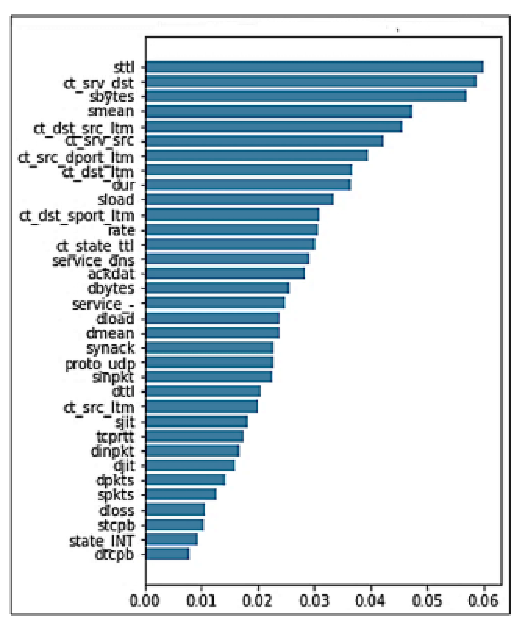
\includegraphics[width=.9\linewidth]{Images/dataset.pdf}
		\caption{
			ویژگی‌های مجموعه داده}
		\label{fig:sumXYPlot}
	\end{figure}
	
	\subsection{طرح پژوهش}
	\subsubsection{
	طبقه‌بند  \lr{Naive Bayes}}
	قضیه بیز و فرض استقلال دو بنیان اصلی هستند که مدل احتمالاتی \lr{Naive Bayes} بر اساس آن‌ها ساخته شده است (ویژگی‌های مورد نظر به یکدیگر بی‌ارتباط هستند). حتی با اینکه سادگی ظاهری آن‌ها ممکن است گمراه‌کننده باشد، مدل‌هایی که تنها با دو برچسب آموزش دیده‌اند، اغلب عملکرد خوبی دارند. جایی که $x$ نمایانگر ویژگی و $C$ کلاسی است که مورد بحث قرار گرفته است. با توجه به این موضوع، سیستم پیشنهادی ممکن است احتمال شرطی $C$ را با استفاده از رابطه بالا، همانطور که در معادله ۱ نشان داده شده است، توصیف کند وقتی $x$ شناخته شده باشد.
	\begin{equation}
		Pr(C | x) = \frac{Pr(x | C)Pr(C)}{Pr(x)}
		\label{eq:bayes}
	\end{equation}
	
	\subsubsection{
		پیش‌بینی طبقه‌بند  \lr{Naive Bayes} براساس احتمالات}
	با توجه به اینکه چهار نوع مختلف از \lr{URL}های مخرب وجود دارد، نرم‌افزار از وزن‌های غیرمضر برای فیلتر کردن آن‌ها استفاده می‌کند. \lr{Naive Bayes} احتمال \lr{PP(CC0)} را به یک \lr{URL} غیرمضر اختصاص می‌دهد و احتمالات \lr{PP(CC1)}، \lr{PP(CC2)}، \lr{PP(CC3)} و \lr{PP(CC0)} را به هر یک از چهار نوع \lr{URL} مخرب اختصاص می‌دهد. احتمال نهایی برای \lr{URL}URL غیرمضر \lr{PP(CC0)} است، در حالی که برای \lr{URL} مخرب، \lr{PP(CC1)} همانطور که در معادلات ۲ و ۳ دیده می‌شود.
	\begin{equation}
		P(C_1) = Pr(C_1) + Pr(C_2) + Pr(C_3) + Pr(C_4)
		\label{eq:probsum}
	\end{equation}
	
	\begin{equation}
		P(C_0) = wPr(C_0)
		\label{eq:scaledprob}
	\end{equation}
	
	\subsection{روش پیشنهادی}
	\subsubsection{انتخاب مناسب‌ترین ویژگی‌ها}
	یک طبقه‌بند \lr{Naive Bayes} به هر ویژگی اعمال خواهد شد تا گروهی با عملکرد بالا شناسایی شود. سپس، پنج ویژگی با بالاترین سطح قابلیت اطمینان انتخاب می‌شوند. سپس طبقه‌بند \lr{Naive Bayes} به صورت تصادفی سه مورد از ویژگی‌های مذکور را انتخاب کرده و از آن‌ها برای قضاوت استفاده می‌کند. نتیجه‌گیری این است که ترکیبی که بالاترین نسبت سود کلی را به همراه دارد، انتخاب شود.
	\subsubsection{استخراج ویژگی}
	در طول این تحقیق، \lr{URL} به روش‌های مختلفی تحلیل و بررسی خواهد شد. داده‌ها ابتدا به شکلی سازماندهی شدند که خواندن آن‌ها آسان‌تر باشد. اولین مجموعه داده‌های ویژگی با بررسی محتوای \lr{URL} و مقایسه بین \lr{URL}های ممکن است مضر و ایمن تولید شد. الگوریتم تکاملی از روشی برای استخراج ویژگی استفاده می‌کند که به ساده‌سازی بردار ویژگی کمک می‌کند، که به نوبه خود سرعت پردازش داده‌ها را افزایش می‌دهد. "الگوریتم ژنتیک (\lr{GA})" اصطلاحی است که در زمینه علوم کامپیوتر برای اشاره به فرآیند تحلیل سیستم‌های بیولوژیکی استفاده می‌شود. روش جستجوی جهانی تصادفی و بهینه‌سازی از محیط طبیعی که فرآیند تکامل در آن صورت می‌گیرد، الهام گرفته شده است. این سیستم بر اساس یک الگوریتم برای جستجوی سریع، کامل و موازی جهانی است.
	
	این رویکرد همه راه‌حل‌های بالقوه را در نظر می‌گیرد و در عین حال از مشکلات مربوط به یک راه‌حل بهینه محلی اجتناب می‌کند. در مقابل، الگوریتم ژنتیک به هیچ وجه توسط ملاحظاتی مانند نیاز به حفظ پیوستگی عملکرد یا شناسایی یک نقطه شروع خاص محدود نمی‌شود. در عوض، الگوریتم ژنتیک آزاد است تا همه نقاط شروع ممکن را بررسی کند و پیوستگی عملکرد را حفظ کند. بهینه‌سازی احتمالاتی نیازی به ایجاد قوانین برای بازیابی و پیمایش خودکار فضای جستجوی بهینه و تنظیم جهت جستجو به عنوان لازم ندارد. این امر به این دلیل ممکن است که بهینه‌سازی احتمالاتی می‌تواند جهت جستجو را به عنوان لازم تطبیق دهد.
	
	فرآیند با بذرگذاری جمعیت، رمزگذاری ویژگی‌ها، و محاسبه تناسب افراد آغاز شد، که در نهایت هر کروموزوم را نمایندگی می‌کردند. این به ما امکان داد تا تعیین کنیم کدام افراد بهترین نماینده برای هر کروموزوم هستند. فرآیند تقاطع برای تولید فرزندان استفاده شد و کروموزوم‌های فرزندان با این مفهوم تغییر یافتند که هرچه فرد مناسب‌تر بود، شانس بهتری برای انتخاب داشت.
	
	روش تقاطع برای تولید فرزندان پس از انتخاب تصادفی دو عضو از جمعیت برای نقش والدین در آزمایش استفاده شد. برای توسعه یک جمعیت جدید، کافی است مراحل روش قبلی را تکرار کنید. در نهایت، سیستم پیشنهادی ممکن است اصلاح شود تا به معیارهای ارزیابی تعیین شده توسط چارچوب‌های مختلف \lr{(TPR، FPR، TNR، FNR)} نزدیک‌تر شود. چهار قانون به ترتیب زیر ارائه می‌شوند:
	
	نرخ مثبت واقعی\lr{(True Positive Rate)} درصدی از موارد بالقوه خطرناک است که با اعمال تحلیل به کل پایگاه داده نمونه‌های مضر شناسایی شده‌اند، همانطور که در معادله \ref{eq:dols} مشاهده می‌شود.
	\begin{equation}
		TP = \frac{N_{M\rightarrow M}}{N_{M\rightarrow M} + N_{M\rightarrow B}}
		\label{eq:dols}
	\end{equation}
	\subsection{نتایج و بحث}
	ارزیابی مجموعه داده‌ها با استفاده از سه روش متمایز انجام شد. پس از تکمیل استانداردسازی داده‌ها، سیستم پیشنهادی به دو مرحله مجزا تقسیم شد: مرحله توسعه و مرحله ارزیابی. برای تعیین برتری نتایج تولید شده توسط یک شبکه عصبی نسبت به مدل استاندار، عملکرد یک مدل رگرسیون لجستیک متعارف به عنوان یک مبنا استفاده می‌شود. بر اساس یافته‌ها همانطور که در جدول ۱ مشاهده می‌شود، امتیاز دقت ۹۶٪، نرخ خطا ۰/۰۴ و امتیاز یادآوری ۹۸٪ است. شناسایی وب‌سایت‌های امن با امتیاز ۹۵٪ موفق است همانطور که در جدول ۲ مشاهده می‌شود. برای تعیین اینکه آیا یک شبکه عصبی می‌تواند در بهبود مسئله کمک کند یا خیر، سیستم پیشنهادی از یک شبکه عصبی استفاده می‌کند. سیستم پیشنهادی ابتدا با استفاده از پیکربندی استاندارد کلاس \lr{SciKit learn} شروع می‌کند و سپس به بررسی گزینه‌های مختلف پیکربندی می‌پردازد تا به حداکثر سطح عملکرد ممکن برسد. نتایج الگوریتم پیشنهادی در جدول ۱ نشان داده شده است.
	%table1
	\begin{table}[H]
		\centering
		\caption{مقایسه تشخیص لینکهای مخرب در روش های گوناگون }
		\begin{tabular}{|l|l|c|c|}
			\hline
			نویسنده & الگوریتم & دقت & خطا \\
			\hline
			Proposed algorithm & Modified NB & 96\% & 0.04 \\
			Moruff Oyelakin \cite{oyelakin2023performance} & DT & 88\% & 0.3 \\
			Subasi \cite{subasi2021comparative} & KNN & 87\% & 0.5 \\
			Jian \cite{jian2016design} & SVM & 91\% & 0.2 \\
			Luo \cite{chen2021malicious} & CNN & 93\% & 0.17 \\
			\hline
		\end{tabular}
	\end{table}
	می‌توان مشاهده کرد که با طبقه‌بندی دو کلاس، ۰ به معنای طبقه‌بندی موفق کلاس‌های غیرمضر و ۱ به معنای طبقه‌بندی لینک‌های مخرب است، همانطور که در جدول ۲ دیده می‌شود.
	%table2
	\begin{table}[H]
		
		\centering
		\label{tab:t}
		\caption{شناسایی وب‌سایت مخرب با استفاده از مدل بیزی چند جمله‌ای}
		\begin{tabular}{|c|c|c|c|c|}
			\hline
			کلاس‌ها & دقت & یادآوری & امتیاز F1 & داده \\
			\hline
			(0) & 0.93 & 0.98 & 0.95 & 630 \\
			(1) & 0.72 & 0.43 & 0.54 & 83 \\
			دقت & 0.90 & 0.90 & 0.91 & 713 \\
			میانگین ماکرو & 0.82 & 0.71 & 0.75 & 713 \\
			وزن‌شده & 0.90 & 0.91 & 0.90 & 713 \\
			\hline
		\end{tabular}
	\end{table}
	
	عملکرد مدل یادگیری ماشین بر روی طبقه‌بندی دودویی به صورت مقایسه‌ای بر روی الگوریتم‌های \lr{Naive Bayes}، درخت تصمیم، \lr{KNN}، رگرسیون لجستیک و جنگل تصادفی در شکل \ref{fig:conclusion} نشان داده شده است. در این آزمایش، \lr{Naive Bayes} به عنوان موفق‌ترین مدل یادگیری ماشین ظاهر شد
	
	
	\subsection{نتیجه گیری}
	شناسایی \lr{URL}های بالقوه مضر یکی از مهم‌ترین فرآیندهای تضمین ایمنی نرم‌افزارهای امنیت سایبری است. دلایلی برای خوش‌بینی در مورد پتانسیل الگوریتم‌های یادگیری ماشین وجود دارد. این مقاله با بررسی استفاده از الگوریتم‌های هوش مصنوعی در فرآیند تعیین اینکه آیا \lr{URL}ها ممکن است حاوی محتوای مخرب باشند یا نه، انجام شد. نتایج نشان می‌دهند که درصد یادآوری ۹۸٪، نرخ دقت ۹۶٪، و نرخ خطا ۰/۰۴ است. در این مطالعه، سیستم پیشنهادی توانست \lr{URL}های بالقوه مضر را با استفاده از رگرسیون لجستیک، شبکه‌های عصبی، و چندین الگوریتم \lr{Naive Bayes} طبقه‌بندی کند. این به ما امکان داد تا تعیین کنیم کدام \lr{URL}ها بیشترین خطر را برای کاربران ایجاد می‌کنند. هنگامی که به مجموعه داده‌های توزیع دشوار اعمال شد، نتایج نشان داد که استراتژی \lr{Naive Bayes} به طور قابل توجهی بهتر از روش‌های رگرسیون لجستیک و شبکه عصبی عمل کرده است.
	
		\begin{figure}
		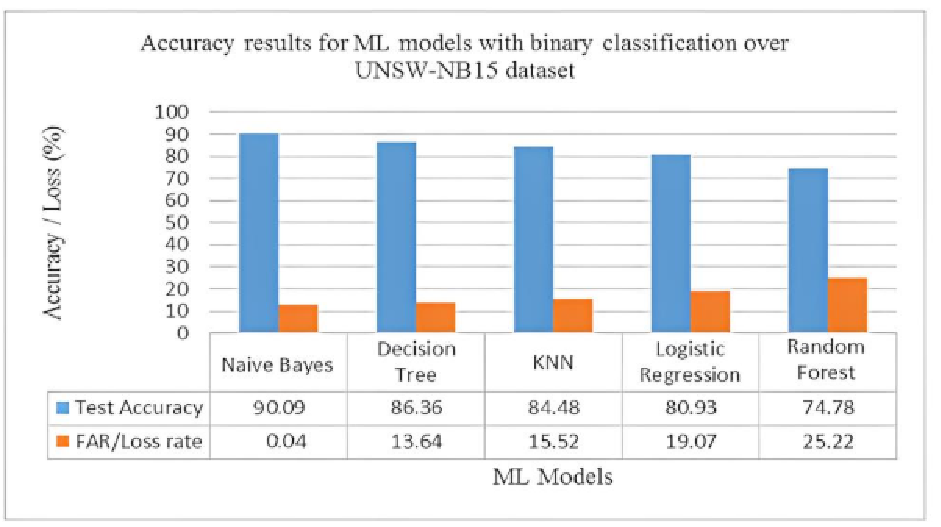
\includegraphics[height=.57\linewidth]{Images/conclusion.pdf}
		\caption{
			عملکرد مدل یادگیری ماشین روی  طبقه‌بندی دودویی}
		\label{fig:conclusion}
	\end{figure}
	
	\section*{پیوست‌ها}
	\bibliography{lib}

\end{document}


